\chapter{Langlands纲领的几何重述之二：阿代尔}\label{L11}\lecturedate{2020/03/23}\sourcepage{89}
已经找到了正规代数簇$X$上$n$维Galois表示的适当替代物：$X$上的秩$n$光滑层，亦即局部系统。以下两个基本事实说明这一替换是合理的。
\begin{enumerate}[label=(\roman*)]
\item 对函数域为$K$的正规代数簇$X$，有$\Gal(K^{\mathrm{ur}}/K)\cong\widehat\pi_1(X,\overline\eta)$，其中$K^{\mathrm{ur}}$为$K$相对于$X$处处非分歧的最大代数扩张。因此，在所有惯性子群上非分歧的Galois表示，可以看作平展基本群$\widehat\pi_1(X)$的表示。
\item 设$X$为连通代数簇，$\overline x$为几何点，$\mathcal F$为$X$上的局部常值层。映射$\mathcal F\mapsto\mathcal F_{\overline x}$给出范畴等价：一侧为茎有限的局部常值集合层（分别地，阿贝尔群层），另一侧为有限连续$\widehat\pi_1(X,\overline x)$集合（分别地，模）。
\end{enumerate}
本讲将进一步讨论光滑层，并为阿代尔寻找适当的几何解释。
\sourcepage{90}
\section{关于光滑层的进一步讨论}\label{L11S1}
上一讲介绍了光滑层，但还不够精确：光滑层是$\ell$进层，一般并不是单个局部常值层。

开头的事实(ii)说明，茎有限的局部常值集合层由平展基本群在几何点处茎上的作用确定。然而，若要把特征0域，例如$\Q$上的向量空间$V$实现为$\widehat\pi_1(X,\overline x)$的表示，就不能仅仅取茎为$V$的离散局部常值层。问题在于需要映射$\widehat\pi_1(X)\to\GL_n(\Q)$连续。$\widehat\pi_1(X)$带有Krull拓扑，开子群都有有限指数。若$\GL_n(\Q)$带有离散拓扑，则连续表示只能具有有限像。
% [Tutor Note: 原书 p90 作 "If we take discrete topology on $\GL_n(\Q)$, then the only continuous map $\widehat\pi_1(X)\to\GL_n(\Q)$ is zero"；但开子群的像必为有限指数，故连续同态的像只能是有限群（可以为零，也可以是有限群），译文已作「连续表示只能具有有限像」。]解决方法是用带$\ell$进拓扑的$\Q_\ell$替代$\Q$，从而把表示构造为某个逆系统的逆极限。因此，这里的局部系统是相容的局部常值层逆系统。为简单起见，只考虑$\Q_\ell$光滑层。

一个\textbf{$\ell$进层}是层的系统$(\mathcal F_n,f_{n+1}:\mathcal F_{n+1}\to\mathcal F_n)_{n\geq1}$，满足：
\begin{enumerate}
\item 对每个$n$，$\mathcal F_n$是$\Z/\ell^n\Z$模的可构造层，即存在有限个局部闭可构造子集组成的分层，使它在每个分层上局部常值且茎为有限生成模；
\item 对每个$n$，$f_{n+1}$诱导同构$\mathcal F_{n+1}/\ell^n\mathcal F_{n+1}\xrightarrow{\sim}\mathcal F_n$。
\end{enumerate}
若所有$\mathcal F_n$均为局部常值层，则这一$\ell$进层称为\textbf{光滑层}。
\originalnumber{1}
\begin{note}[L11S1O1]
有时术语略作混用，称光滑层为“局部常值$\ell$进层”；但一般不能通过一个平展覆盖同时将整个逆系统平凡化。
\end{note}
\originalnumber{2}
\begin{example}\label{L11S1O2}\idx{Tate层}\idx{Tate扭转}\idx{分圆特征标}
设$k$为域，$\mu_n$为$n$次单位根的有限群层。$\Spec k$上的Tate层\znote{Tate层 $\Z_\ell(r)$ 是 $\ell$ 进意义下的 $r$ 次扭转：它把单位根层 $\mu_{\ell^n}^{\otimes r}$ 按 $\ell$ 的幂排成逆系统，对应的连续表示正是分圆特征标的 $r$ 次幂。它在几何中扮演「上同调平移」的角色，许多簇的上同调群之间的扭转关系都用这一记号表达；不同文献的符号约定可能整体相差一个符号（$r$ 与 $-r$ 互换）。[来源：nLab "Tate twist"，\url{https://ncatlab.org/nlab/show/Tate+twist}（Last revised 2025-08-10；2026-11-14 访问）。]}
\[\Z_\ell(r):=(\mu_{\ell^n}^{\otimes r},\ f_{n+1}:\mu_{\ell^{n+1}}^{\otimes r}\to\mu_{\ell^n}^{\otimes r})_{n\geq1}\]
是光滑的，其中$\ell\ne\operatorname{char}(k)$。取相容本原单位根$\zeta_{\ell^{n+1},j}^\ell=\zeta_{\ell^n,j}$，则过渡映射为
\[f_{n+1}:\bigotimes_{j=1}^r\zeta_{\ell^{n+1},j}^{k_j}\longmapsto\bigotimes_{j=1}^r\zeta_{\ell^n,j}^{k_j}.\]
\sourcepage{91}
注意，本原单位根$\zeta_{\ell^n,j}$（$1\leq j\leq r$）给出$r$个同构$\mu_{\ell^n}\cong\Z/\ell^n\Z$，并且$\mu_{\ell^{n+1}}/\ell^n\mu_{\ell^{n+1}}\cong\mu_{\ell^n}$。

Tate层$\Z_\ell(r)$对应于连续表示
\[\Gal(k^{\mathrm{sep}}/k)\longrightarrow\Gal(k(\mu_{\ell^\infty})/k)\hookrightarrow\Z_\ell^\times\longrightarrow\operatorname{Aut}_{\Z_\ell}(\Z_\ell(r)_{\overline x}),\]
其中最后的箭头为取$r$次幂。有
\[\begin{aligned}
\operatorname{Aut}_{\Z_\ell}(\Z_\ell(r)_{\overline x})
&=\{(\xi_n)\mid\xi_n\in\operatorname{Aut}(\mu_{\ell^n}^{\otimes r}),\ f_{n+1}\xi_{n+1}=\xi_nf_{n+1}\}\\
&\cong\Z_\ell^\times.
\end{aligned}\]
因此，$\Z_\ell(r)$对应于分圆特征标的$r$次幂。显式地，若$\sigma(\zeta_{\ell^n,j})=\zeta_{\ell^n,j}^{m(n)}$，则$\chi_\ell(\sigma)=\varprojlim_nm(n)\in\Z_\ell^\times$，而$\sigma$在张量幂上的作用为
\[\chi_\ell(\sigma)^r\in\GL_1(\Z_\ell).\]
% [Tutor Note: 原书 p91 把 $\operatorname{Aut}_{\Z_\ell}(\Z_\ell(r)_{\overline x})$ 写成 $(\Z_\ell^\times)^{\otimes r}$ 型逆极限，并把 $\sigma$ 的作用写成 $Diag(\varprojlim m_1(n),\dots,\varprojlim m_r(n))\in(\Z_\ell^\times)^{\otimes r}\subset\GL_r(\Z_\ell)$；因 $\Z_\ell(r)$ 是秩 1 光滑层，自同构群应为 $\Z_\ell^\times$，作用为分圆特征标的 $r$ 次幂 $\chi_\ell(\sigma)^r\in\GL_1(\Z_\ell)$，译文已按此处理。同页原书还作 $\Gal(k(\zeta_{\ell^n})/k)\cong\Z_\ell^\times$，译文改为 $\Gal(k(\mu_{\ell^\infty})/k)\hookrightarrow\Z_\ell^\times$。]
\end{example}
有限自由$\Z_\ell$模的光滑层实际上对应于连续表示$\widehat\pi_1(X)\to\GL_r(\Z_\ell)$。形式地将其系数与$\Q_\ell$张量，就得到$\Q_\ell$光滑层。

再介绍光滑层的平展上同调。上同调一般不与层的逆极限交换。在上同调有限的情形，对$X$上的光滑层$\mathcal F=(\mathcal F_n)$，定义
\[H^r_{\mathrm{ét}}(X,\mathcal F):=\varprojlim_nH^r_{\mathrm{ét}}(X,\mathcal F_n).\]
也可以将其与$\Q_\ell$形式张量，得到$\Q_\ell$向量空间；有时仍将这一向量空间记为$H^r_{\mathrm{ét}}(X,\mathcal F)$。

平展拓扑比Zariski拓扑更细，因此，即使概形在Zariski拓扑中不可约，其有限系数局部常值层仍可具有非平凡平展上同调。
\originalnumber{3}
\begin{theorem}\label{L11S1O3}
若$X$为不可约拓扑空间，则对任意常值阿贝尔群层$\Lambda$及所有$r>0$，都有$H^r(X,\Lambda)=0$。
\end{theorem}
\begin{proof}因为$\Lambda$是松弛层。\end{proof}
在平展拓扑中，非平凡局部常值层并不具有上述松弛性质。可以取两个平展覆盖$Y_j\to X$的无交并
\sourcepage{92}
$Y_1\sqcup Y_2$，它仍为平展覆盖，但非平凡常值层的限制映射$\Lambda(X)\to\Lambda(Y_1\sqcup Y_2)=\Lambda(Y_1)\times\Lambda(Y_2)$只有对角像，不能满射。下面两个例子有助于理解平展拓扑相对于Zariski拓扑的优势。
\originalnumber{4}
\begin{example}\label{L11S1O4}\idx{Kummer正合列}
设$X$为$k$上的代数簇，$\OO_X^\times$为处处非零正则函数组成的层。取与$\operatorname{char}(k)$互素的正整数$n$。取$n$次幂诱导层态射
\begin{equation}\tag{1.1}\label{L11eq11}
\OO_X^\times\xrightarrow{\ f\mapsto f^n\ }\OO_X^\times.
\end{equation}
这一态射在Zariski拓扑中一般不满射，在平展拓扑中却满射。为简单起见，在$X=\C^\times$的情形解释。只需证明每个点$x$处的茎映射$\OO_{X,\overline x}^\times\xrightarrow{t\mapsto t^n}\OO_{X,\overline x}^\times$满射。对$t\in\OO_{X,\overline x}^\times$，存在平展态射$U\to X$，使$t$可由$U$上的可逆正则函数代表。由$t$给出映射$U\to\C^\times$，拉回$n$次平展覆盖$\C^\times\to\C^\times$，$x\mapsto x^n$，得到Cartesian图：
\begin{figure}[H]\centering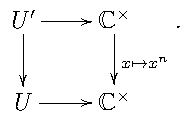
\includegraphics[width=0.1535\paperwidth]{images/L11-p092-Kummer.pdf}\end{figure}
于是$U'$仍为$x$的平展邻域，且有$\tau\in\OO_{U'}^\times$满足$\tau^n=t$。
\end{example}
\originalnumber{5}
\begin{example}\label{L11S1O5}
设$\mu_n$为$n$次单位根层，它是局部常值层。下面说明当$n>1$时，$H^1_{\mathrm{ét}}(\C^\times,\mu_n)\ne0$。利用\eqref{L11eq11}的满射得到上同调长正合列：
\begin{figure}[H]\centering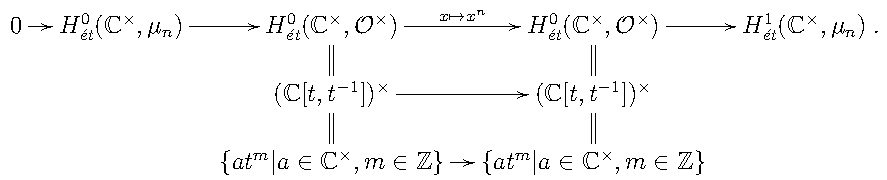
\includegraphics[width=0.7152\paperwidth]{images/L11-p092-cohomology.pdf}\end{figure}
映射$(\C[t,t^{-1}])^\times\to(\C[t,t^{-1}])^\times$，$at^m\mapsto a^nt^{mn}$，不满射，余核为$\Z/n\Z$，故$H^1_{\mathrm{ét}}(\C^\times,\mu_n)\ne0$。事实上，$H^1_{\mathrm{ét}}(\C^\times,\mu_n)\cong\Z/n\Z$。
\end{example}
\originalnumber{6}
\begin{theorem}{比较定理}\label{L11S1O6}
设$X$为$\C$上的非奇异代数簇。对任意有限阿贝尔群$\Gamma$及$r\geq0$，有$H^r_{\mathrm{ét}}(X,\Gamma)\cong H^r(X^{\mathrm{an}},\Gamma)$，其中$X^{\mathrm{an}}$为把$X$看作复流形所得的解析空间。
\end{theorem}
\sourcepage{93}
\section{阿代尔与向量丛}\label{L11S2}\idx{向量丛}\idx{除子}
先回顾两个代数事实。
\begin{itemize}
\item 若$\OO$为整闭整环，则$\OO=\bigcap_{\operatorname{ht}(\p)=1}\OO_{\p}$。
\item 若$\OO$为这样的整环，分式域为$F$，则序列
\[1\to\OO^\times\to F^\times\xrightarrow{\oplus_{\p}\ord_{\p}}\bigoplus_{\operatorname{ht}(\p)=1}\Z\to0\]
正合，当且仅当$\OO$为唯一分解整环，即UFD\znoteplain{原书此处只作「整闭整环」（integrally closed integral domain），未假定 Noether 性；而「$\OO$ 等于各高度 1 素理想局部化之交」与该序列正合 $\Leftrightarrow$ UFD 这两条事实，通常在 Noether 整闭整环（或 Krull 环）上陈述。阅读时须自行补上 Noether 假设，否则第一条事实（Krull 交定理）一般不成立；正文仍按原书处理。（上下文推断，无外部依据）}。
\end{itemize}
\originalnumber{1}
\begin{proposition}\label{L11S2O1}
设$X$为非奇异代数簇，则$X$上有层的正合列
\[1\to\OO_X^\times\to\mathcal F^\times\to\operatorname{Div}\to0,\]

\end{proposition}
设$X$为光滑代数曲线，$F$为其函数域。每个闭点$v\in X$给出$F$的一个离散赋值，局部环为UFD。这里用$\OO_x$表示其完备赋值环，$F_x$表示局部完备化。给定除子$D=\sum_{x\in|X|}n_x[x]$，由\eref{命题}{L11S2O1}，它在每个$x$处确定$F_x^\times$中$\OO_x^\times$的一个陪集$D_x\OO_x^\times$；当$n_x=0$时，该陪集就是$\OO_x^\times$。于是，$I_F/\prod_x\OO_x^\times$恰为$X$上的除子群。主除子对应于$F^\times$的元素，因此双商$F^\times\backslash I_F/\prod_x\OO_x^\times$是除子类群，也就是$X$上线丛同构类组成的群。

令$B=\prod_x\OO_x$为$\A_F$的最大紧加法子群，并令$K=\GL_n(B)$。一般地有以下结论。
\originalnumber{2}
\begin{theorem}\label{L11S2O2}
集合$\GL_n(F)\backslash\GL_n(\A_F)/K$与$X$上秩$n$向量丛的同构类集合之间存在双射。
\end{theorem}
\begin{proof}
可以按下述方式证明。对任意秩$n$向量丛$\mathcal V$，存在泛纤维的平凡化$T_X:\mathcal V\otimes_{\OO_X}F\xrightarrow{\sim}F^n$，并且对所有闭点$x$，存在局部平凡化$t_x:\OO_x^n\xrightarrow{\sim}\mathcal V\otimes_{\OO_X}\OO_x$。
\sourcepage{94}
于是有下图：
\begin{figure}[H]\centering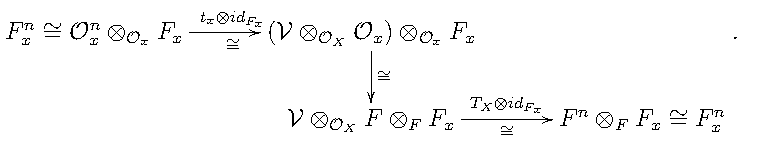
\includegraphics[width=0.6202\paperwidth]{images/L11-p094-trivialization.pdf}\end{figure}
对每个$x$，这给出元素$\mathcal V(x)\in\GL_n(F_x)$。由于$T_X$在几乎所有$x$处都诱导整平凡化，几乎所有$\mathcal V(x)$均属于$\GL_n(\OO_x)$，因此$(\mathcal V(x))_x\in\GL_n(\A_F)$。改变$T_X$或$t_x$，分别相当于在左边乘以$\GL_n(F)$中的元素，或在右边乘以$K$中的元素。
\end{proof}
现在，已为集合$\GL_n(F)\backslash\GL_n(\A_F)/K$找到几何解释，但这还不够。希望为所有秩$n$向量丛\znote{向量丛是「局部自由模」的几何版本：$X$ 上的秩 $n$ 向量丛即局部同构于 $\OO_X^{\oplus n}$ 的 $\OO_X$ 模层，等价于 $\GL_n$ 主丛（选定标架后）。在光滑曲线上，它与双商 $\GL_n(F)\backslash\GL_n(\A_F)/K$ 的同构类一一对应（定理 2.2），这是阿代尔语言与几何语言之间的桥；不做刚性化就得不到概形参数空间，只能得到模叠 $\operatorname{Bun}_n(X)$。[来源：nLab "vector bundle"，\url{https://ncatlab.org/nlab/show/vector+bundle}（Last revised 2025-10-21；2026-11-14 访问）。]}的同构类集合$\operatorname{Bun}_n(X)$赋予更多结构。可以考虑它是否由一个概形表示，但保留所有向量丛及其族的这一模问题不能直接由概形表示。要得到向量丛的参数空间，有两条途径：一是取概形形式的粗模空间，只参数化半稳定丛的$S$等价类；二是取模叠，参数化所有丛。下面采用第二条途径。
\section{模叠}\label{L11S3}\idx{模叠}\idx{代数叠}
已经看到，$\GL_n(F)\backslash\GL_n(\A_F)/K$与$\operatorname{Bun}_n(X)$中的同构类一一对应。因此，在Langlands纲领的几何表述中，用$\operatorname{Bun}_n(X)$替代这一双商。不过，$\operatorname{Bun}_n(X)$是叠，而不是概形。

叠源于模问题。对模函子而言，最理想的情形是它可以由概形表示，但这种情形并不常见。主要障碍是待参数化对象具有非平凡自同构。有时可以给对象添加额外结构，强制自同构群平凡，这称为将函子\textbf{刚性化}。例如，在固定点$x\in X$处，给每条线丛$\mathcal L$添加一个标架$\mathcal L_x\cong k$，
\sourcepage{95}
即可使次数0的线丛模问题由Jacobian概形$J(X)$表示。不过，一般模函子的刚性化可能十分复杂，并过度改变原有模问题。因此使用模叠\znote{模叠用群胚值函子记录模问题：把每个测试概形 $S$ 送去 $S$ 上的一族对象构成的群胚，从而保留对象的自同构，而不像粗模空间那样把它们压掉。代价是它只在 2 范畴意义下存在，需用 fppf 下降来陈述层性质（本节 (i)(ii) 两条）。$\operatorname{Bun}_n(X)$ 是典型例子：它不能由概形表示，但作为代数叠可由 Quot 概形的商叠局部覆盖（注 3.3）。[来源：nLab "moduli stack"，\url{https://ncatlab.org/nlab/show/moduli+stack}（Last revised 2023-04-16；2026-11-14 访问）。]}来代替概形，保留对象的全部自同构。

设$k$为基域。$k$概形$S$可看成反变函子$\underline S:(\mathrm{Sch}/k)\to(\mathrm{Sets})$，$T\mapsto\Hom(T,S)$。$S\cong S'$当且仅当$\underline S\cong\underline S'$。

一个$k$叠$\mathfrak X$首先是群胚值反变伪函子
\[\mathfrak X:(\mathrm{Sch}/k)\to(\mathrm{Gpds}),\]
其中群胚是所有态射均为同构的范畴。$(\mathrm{Gpds})$是2范畴：对两个群胚$G_1,G_2$，$\operatorname{Mor}_{\mathrm{Gpds}}(G_1,G_2)$本身也是范畴。对$S\xrightarrow f S'\xrightarrow g S''$，有三个群胚$\mathfrak X(S)$、$\mathfrak X(S')$、$\mathfrak X(S'')$，而下图仅在2范畴意义下交换：
\begin{figure}[H]\centering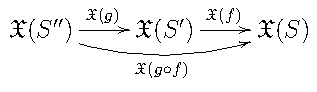
\includegraphics[width=0.2556\paperwidth]{images/L11-p095-pseudofunctor.pdf}\end{figure}
也就是说，有典范的函子同构$\alpha_{f,g}:\mathfrak X(g\circ f)\xrightarrow{\sim}\mathfrak X(f)\circ\mathfrak X(g)$。这些同构满足余循环条件：对可复合的$f,g,h$，
\[(\mathfrak X(f)\alpha_{g,h})\circ\alpha_{f,h\circ g}=(\alpha_{f,g}\mathfrak X(h))\circ\alpha_{g\circ f,h},\]
两边都是从$\mathfrak X(h\circ g\circ f)$到$\mathfrak X(f)\mathfrak X(g)\mathfrak X(h)$的自然同构。这样的函子也称为伪函子。
% [Tutor Note: 原书 p95 称这类函子为 "lax functors"，但此处要求比较同构 $\alpha_{f,g}$ 可逆、且只在 2 范畴意义下交换，按通行术语应称伪函子（pseudofunctor）；译文已作「伪函子」。]要成为$k$叠，还须满足以下两个条件。
\begin{enumerate}[label=(\roman*)]
\item 对每个$k$概形$S$及$x,y\in\operatorname{Ob}(\mathfrak X(S))$，函子
\[\begin{aligned}
\underline{\operatorname{Isom}}(x,y):\mathrm{Sch}/S&\to\mathrm{Sets},\\
(T\xrightarrow f S)&\longmapsto\Hom_{\mathfrak X(T)}(\mathfrak X(f)(x),\mathfrak X(f)(y))
\end{aligned}\]
\idx{fppf}在fppf拓扑中为层。即对任意忠实平坦且有限表现的覆盖族$\{U_i\to U\}$，有等化子序列
\[\underline{\operatorname{Isom}}(x,y)(U)\to\prod_i\underline{\operatorname{Isom}}(x,y)(U_i)\rightrightarrows\prod_{i,j}\underline{\operatorname{Isom}}(x,y)(U_{ij}),\]
其中$U_{ij}:=U_i\times_UU_j$。
\sourcepage{96}
\item 每个下降数据都有效。

对覆盖族$\{U_i\to U\}$，一个\textbf{下降数据}\znote{下降数据给「在覆盖上给出局部对象、再用同构粘起来」一个形式化：$(x_i,\varphi_{ij})$ 记录局部对象与转移同构，余循环条件保证三次交叠上相容；「有效」是说确实存在整体对象把它们粘合。叠的公理 (ii) 要求每个下降数据有效，这正是「层」条件在群胚值层面的推广，也说明了为何模叠要用 fppf 拓扑而非 Zariski 拓扑。[来源：nLab "descent"，\url{https://ncatlab.org/nlab/show/descent}（Last revised 2024-09-12；2026-11-14 访问）。]}是一族$(x_i,\varphi_{ij})$，其中$x_i\in\operatorname{Ob}(\mathfrak X(U_i))$，$\varphi_{ij}$为$\mathfrak X(U_{ij})$中的同构
\[\varphi_{ij}:x_i|_{U_{ij}}\xrightarrow{\sim}x_j|_{U_{ij}},\]
并在$U_{ijk}:=U_i\times_UU_j\times_UU_k$上满足余循环条件$\varphi_{jk}\circ\varphi_{ij}=\varphi_{ik}$。下降数据\textbf{有效}，是指存在$x\in\operatorname{Ob}(\mathfrak X(U))$及同构$\varphi_i:x|_{U_i}\xrightarrow{\sim}x_i$，使在$U_{ij}$上有$\varphi_j=\varphi_{ij}\circ\varphi_i$。
% [Tutor Note: 原书 p96 的余循环条件作 $\varphi_{ki}|_{U_{kji}}=\varphi_{kj}\circ\varphi_{ji}$，而 $U_{kji}:=U_k\times_UU_j\times_UU_i$，下标与 $U_{ijk}$ 的定义错位；译文按标准写法 $\varphi_{jk}\circ\varphi_{ij}=\varphi_{ik}$ 处理，二者在重排三元组下标后等价。]
\end{enumerate}
\idx{下降数据}
\originalnumber{1}
\begin{note}[L11S3O1]
fppf是法语“fidèlement plat et de présentation finie”的缩写，意为“忠实平坦且有限表现”。有时还会见到fpqc，它来自“fidèlement plat et quasi-compact”，意为“忠实平坦且拟紧”。
\end{note}
对任意$k$概形$S$及$\kappa\in\mathfrak X(S)$，并对$k$概形$U$上的对象$\eta\in\mathfrak X(U)$，定义$U$叠$U_\eta(\kappa)$如下：
\[\begin{aligned}
U_\eta(\kappa):\mathrm{Sch}/U&\longrightarrow\mathrm{Gpds},\\
(T\xrightarrow f U)&\longmapsto\{(\xi,\alpha)\mid\xi\in\Hom(T,S),\ \alpha:\mathfrak X(\xi)(\kappa)\xrightarrow{\sim}\mathfrak X(f)(\eta)\}.
\end{aligned}\]
其纤维化范畴中的态射$(\xi,\alpha)$到$(\xi',\alpha')$由$U$上的映射$h:T\to T'$给出，满足$\xi=\xi'\circ h$，且在相容的拉回同构下$\alpha=h^*\alpha'$。
% [Tutor Note: 原书 p96 定义 $U_\eta(\kappa)$ 时写 $h\in\Hom(T,T)$，但条件 $\xi=\xi'\circ h$（$\xi:T\to S$，$\xi':T'\to S$）要求 $h:T\to T'$，应为 $\Hom(T,T')$；译文按 $T\to T'$ 处理。]可把$\kappa$看成映射$\underline S\to\mathfrak X$，于是有Cartesian图：
\begin{figure}[H]\centering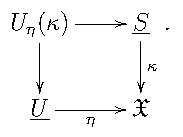
\includegraphics[width=0.1475\paperwidth]{images/L11-p096-fiber.pdf}\end{figure}
若对任意$S,\kappa,U,\eta$，$U_\eta(\kappa)$均由概形表示，并且存在$k$概形$P$及$p\in\mathfrak X(P)$，使每个基变换$U_\eta(p)\to U$均为光滑满射，则称$\mathfrak X$为代数叠。
\originalnumber{2}
\begin{theorem}\label{L11S3O2}
设$X$为连通完备光滑曲线，则$\operatorname{Bun}_n(X)$是代数叠。
\end{theorem}
\sourcepage{97}
\originalnumber{3}
\begin{note}[L11S3O3]
叠$\operatorname{Bun}_n(X)$可由参数化局部自由商$\OO_X(m)^N\twoheadrightarrow\mathcal E$的Quot概形$Q_{m,N}:=\operatorname{Quot}(\OO_X(m)^N)^{\mathrm{lf}}$中的适当开子概形覆盖。不过，不能用有限多个这样的$Q_{m,N}$覆盖全部$\operatorname{Bun}_n(X)$，因此它只是局部有限型。局部选取适当的Quot开集后，$\operatorname{Bun}_n(X)$同构于商叠$[Q_{m,N}/\GL_N]$。商叠$[Z/H]$的维数定义为$\dim Z-\dim H$。写作$\operatorname{Bun}_n(X)=\coprod_d\operatorname{Bun}_n^d(X)$，其中$\operatorname{Bun}_n^d(X)$参数化秩$n$、次数$d$的向量丛。每个这样的叠都是有限维的，尽管$n\geq2$时一般并非有限型。

若$\dim X=M\geq2$，则当$n>1$时，参数化秩$n$、Chern类$(c_1,\ldots,c_M)$向量丛的叠$\operatorname{Bun}_{n,c_1,\ldots,c_M}(X)$一般为无限维。
\end{note}
\needspace{5\baselineskip}\section{第11讲参考文献}\label{L11S4}
\needspace{4\baselineskip}\textbf{关于平展上同调。}
\begin{references}
\refitem{L11bibM}{M} J. S. Milne, \emph{Lectures on étale cohomology}, Course notes. pp. 1-202. \url{http://www.jmilne.org/math/CourseNotes/CFC.pdf}.
\end{references}
\needspace{4\baselineskip}\textbf{关于叠。}
\begin{references}
\refitem{L11bibS}{S} Ch. Sorger, \emph{Lectures on moduli of principal G-bundles over algebraic curves}, in \emph{School on algebraic geometry} (Trieste, 1999), ICTP Lecture Notes 1, ICTP, Trieste, pp. 1-57, available at \url{http://www.ictp.trieste.it/~pub_off/lectures}.
\end{references}
